%%%%%%%%%%%%%%%%%%%%%%%%%%%%%%%%%%%%%%%%%
% Large Colored Title Article
% LaTeX Template
% Version 1.1 (25/11/12)
%
% This template has been downloaded from:
% http://www.LaTeXTemplates.com
%
% Original author:
% Frits Wenneker (http://www.howtotex.com)
%
% License:
% CC BY-NC-SA 3.0 (http://creativecommons.org/licenses/by-nc-sa/3.0/)
%
%%%%%%%%%%%%%%%%%%%%%%%%%%%%%%%%%%%%%%%%%

%
%	JC: POR FAVOR, NO MODIFIQUEN EL FORMATO DEL DOCUMENTO.
%
%----------------------------------------------------------------------------------------
%	PACKAGES AND OTHER DOCUMENT CONFIGURATIONS
%----------------------------------------------------------------------------------------

\documentclass[DIV=calc, 
					paper=letter, 
					fontsize=11pt, 
					twocolumn]{scrartcl}

\usepackage{lipsum}
\usepackage[spanish]{babel}
\usepackage[protrusion=true,
				expansion=true]{microtype}
\usepackage{amsmath,amsfonts,amsthm}
\usepackage[svgnames]{xcolor}
\usepackage[hang, small,labelfont=bf,up,textfont=it,up]{caption}
\usepackage{booktabs}
\usepackage{fix-cm}
\usepackage{graphicx}

\usepackage{sectsty}
\allsectionsfont{\usefont{OT1}{phv}{b}{n}} % Change the font of all section commands

\usepackage{fancyhdr}
\pagestyle{fancy}
\usepackage{lastpage}

% Headers - all currently empty
\lhead{}
\chead{}
\rhead{}

% Footers
\lfoot{}
\cfoot{}
\rfoot{\footnotesize P\'agina \thepage\ de \pageref{LastPage}} % "Page 1 of 2"

\renewcommand{\headrulewidth}{0.0pt}
\renewcommand{\footrulewidth}{0.4pt}

\usepackage{lettrine} % Package to accentuate the first letter of the text
\newcommand{\initial}[1]{ % Defines the command and style for the first letter
\lettrine[lines=3,lhang=0.3,nindent=0em]{
\color{DarkGoldenrod}
{\textsf{#1}}}{}}

%----------------------------------------------------------------------------------------
%	TITLE SECTION
%----------------------------------------------------------------------------------------

\usepackage{titling} % Allows custom title configuration
\newcommand*{\addheight}[2][.5ex]{%
  \raisebox{0pt}[\dimexpr\height+(#1)\relax]{#2}%
}
\newcommand{\HorRule}{\color{DarkGoldenrod} \rule{\linewidth}{1pt}} % Defines the gold horizontal rule around the title

\pretitle{\vspace{-30pt} \begin{flushleft} \HorRule \fontsize{50}{50} \usefont{OT1}{phv}{b}{n} \color{DarkRed} \selectfont} % Horizontal rule before the title

%
%	JC: ADAPTAR
%
\title{\Huge Reporte ACT-11302} % Your article title

\posttitle{\par\end{flushleft}\vskip 0.5em} % Whitespace under the title

\preauthor{\begin{flushleft}\large \lineskip 0.5em \usefont{OT1}{phv}{b}{sl} \color{DarkRed}} % Author font configuration

\author{	Lorena Piedras Saenz \ \ \ 
			\& \ \ \ 
			Guillermo Santiago Novoa P\'erez\ \ }

\postauthor{\footnotesize 
				\usefont{OT1}{phv}{m}{sl} 
				\color{Black}
				% Configuration for the institution name
				ITAM % Your institution

\par\end{flushleft}\HorRule} % Horizontal rule after the title

\date{\today} % Add a date here if you would like one to appear underneath the title block

%----------------------------------------------------------------------------------------

\begin{document}

\maketitle % Print the title

\thispagestyle{fancy} % Enabling the custom headers/footers for the first page 

%----------------------------------------------------------------------------------------
%	ABSTRACT
%----------------------------------------------------------------------------------------

% The first character should be within \initial{}
\initial{E}\textbf{n la pr\'actica actuarial, el modelamiento, medici\'on y control de la capacidad de una empresa de seguros para pagar sus obligaciones son algunas de las actividades que m\'as preocupaci\'on causan. Las razones de esto son bastante l\'ogicas dado que si una aseguradora no puede pagar sus obligaciones, su operaci\'on perder\'ia todo el sentido.  En este proyecto se intentar\'a predecir la distribuci\'on de accidentes automovil\'isticos a la que se enfrentar\'a una compa\~{n}\'ia aseguradora en los a\~{n}os 2008 y 2009 con informaci\'on de siniestros de los tres a\~{n}os anteriores. De la misma manera, propondremos una prima que, de acuerdo a nuestra predicci\'on, le deje a la aseguradora mantenerse en el mercado de manera competitiva.}

%----------------------------------------------------------------------------------------
%	ARTICLE CONTENTS
%----------------------------------------------------------------------------------------
%----------------------------------------------------------------------------------------
%	ARTICLE CONTENTS
%----------------------------------------------------------------------------------------

\section{An\'alisis Exploratorio de los Datos}

\indent Trataremos a nuestros datos qued\'andonos con los asegurados que tuvieron al menos un siniestro. Este cambio se lo realizaremos a la base de datos \" \ All State DataClaims\" \ que se encuentra en un concurso de kaggle.
%\lipsum*

\begin{table}[h*]
\caption{Cuartiles datos positivos}
\centering
\resizebox{0.4\textwidth}{!}
{
\begin{tabular}{ccccc|l}
\toprule
Min & 1st Qu. & Median & 3rd Qu. & Max & Mean\\
\midrule
$0.003$ & $10.190$ &$37.130$ &$140.0$ &$6422.0$ & $171.3$ \\
\bottomrule
\end{tabular}}
\end{table}
\noindent De entrada podemos ver que estamos tratando con datos que tienen cola derecha extremadamente pesadas. Esto se muestra tanto en el histograma de los mismos como en los estad\'isticos cotidianos de exploraci\'on de datos.
\begin{tabular}{|c|}
      \hline
      \addheight{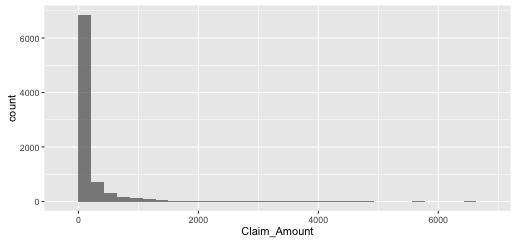
\includegraphics[width=75mm]{hist_posit.png}} \\
      \hline
\end{tabular}
%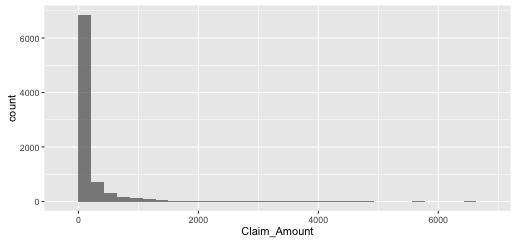
\includegraphics[trim = 0mm 0mm 00mm 0mm, clip, scale=\textwidth]{hist_posit.png}\\
%\begin{align}
%A = 
%\begin{bmatrix}
%A_{11} & A_{21} \\
%A_{21} & A_{22}
%\end{bmatrix}
%\end{align}

%\lipsum[4] % Dummy text

%------------------------------------------------

\subsection{Separaci\'on por a\~{n}o}

\indent Pensamos separar los datos por a\~{n}o dado que, tanto el n\'umero de asegurados como la intensidad de siniestros, presentan cierta tendencia a\~{n}o a a\~{n}o.\\
\begin{tabular}{|c|}
      \hline
      \addheight{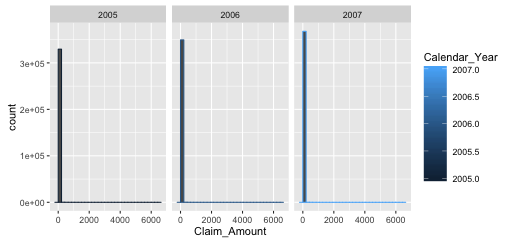
\includegraphics[width=60mm]{claim_amount_anual_cero.png}} \\
      \addheight{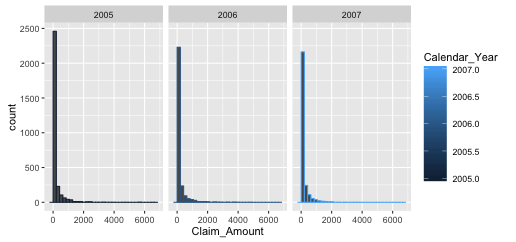
\includegraphics[width=60mm]{claim_amount_anual.png}} \\
      \addheight{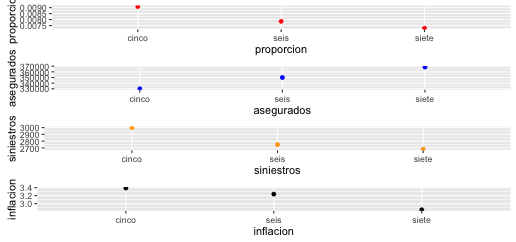
\includegraphics[width=60mm]{datos_anuales_N.png}} \\
      \hline
\end{tabular}
%\lipsum[5] % Dummy text

\begin{itemize}
\item Tambi\'en podemos notar una tendencia en la inflaci\'on (EEUU), sin embargo trataremos con ella como si fuera algo independiente a los asegurados y al n\'umero de siniestros (por facilidad).
\item La tendencia que existe en el total de asegurados con un siniestro lo trataremos como una tendencia en la intensidad de un proceso Poisson, el cu\'al trataremos tambi\'en de manera independiente al costo de cada siniestro.
\item Utilizaremos un modelo colectivo para el costo total de los siniestros en cada a\~{n}o.
\item El hecho de que estemos asumiendo independencia tambi\'en se basa en que, como no conocemos la estructura de cualquier dependencia que haya (por ejemplo, que crezca el n\'umero de asegurados pero baje el n\'umero de siniestros), podr\'iamos caer en una trampa y sobreajustar en nuestro modelo.
\end{itemize}

%\lipsum[6] % Dummy text

%------------------------------------------------

\subsection{Separaci\'on por Variables}
\begin{tabular}{|c|}
	\hline
  	\addheight{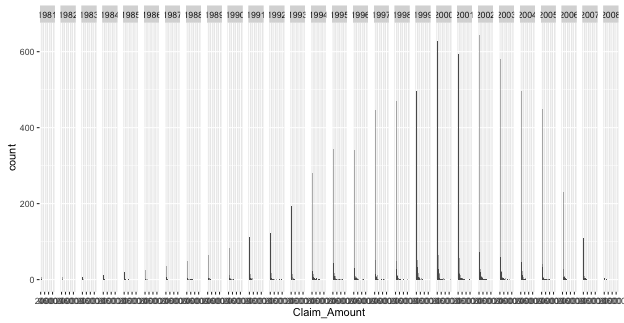
\includegraphics[width=75mm]{claim_amount_model.png}}\\
	\hline
\end{tabular}
\noindent En la tabla anterior se muestran diferentes gr\'aficas de barras si separ\'aramos el modelo en un modelo por cada a\~{n}o del modelo del carro que tuvo un siniestro. En el concurso de kaggle especifican que tomar las variables extras (las que no son el costo del siniestro) para intentar explicar los costos no es buena idea, sin embargo indican que tal vez mezclar ciertas variables pueda ayudar a clasificar los costos. El problema de este enfoque est\'a en que, simplemente tomando una variable para clasificar ya tendr\'iamos m\'as de 80 diferentes modelos, todav\'ia nos faltar\'ia encontrar qu\'e interacciones podr\'ian ayudar a clasificar y tomar el n\'umero total de modelos resultantes. Esto resultar\'ia en demasiados modelos y perder\'iamos la facilidad de explicar qu\'e est\'a pasando (una parte muy importante en nuestra visi\'on del riesgo de la aseguradora); por lo tanto, aunque encontrar esas relaciones entre variables sea un tema interesante, parece estar fuera de nuestro enfoque y no lo abordaremos en este trabajo.

%------------------------------------------------

\section{Ajuste y Selecci\'on de Modelos}
\indent Habiendo decidido separar nuestro modelo por a\~{n}o, ahora nos enfocaremos en ajustar una distribuci\'on el costo de los siniestros de cada a\~{n}o. Como vimos en el an\'alisis descriptivo de los datos, parece ser que los siniestros siguen una distribuci\'on de colas pesadas, por lo que utilizaremos dos paquetes para encontrar estas distribuciones (fExtremes, evdbayes) y despu\'es intentaremos aplicar alg\'un criterio para seleccionar qu\'e modelo se ajusta mejor a nuestros datos.\\
\subsection{Enfoque frecuentista}
\indent {\small{Para el primer enfoque utilizaremos el paquete fExtremes de R adem\'as de otros paquetes como ggplot2 para graficar los resultados. }}
%\lipsum[8] % Dummy text
\begin{tabular}{|cc|}
      \hline
      \addheight{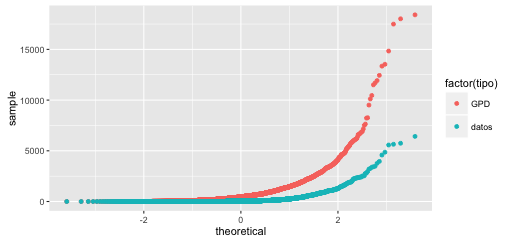
\includegraphics[width=35mm]{5gevf.png}} &
      \addheight{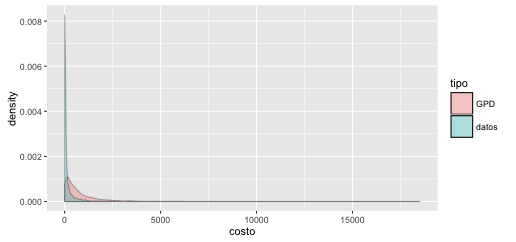
\includegraphics[width=35mm]{5gevf_dens.png}} \\
      \hline
      \addheight{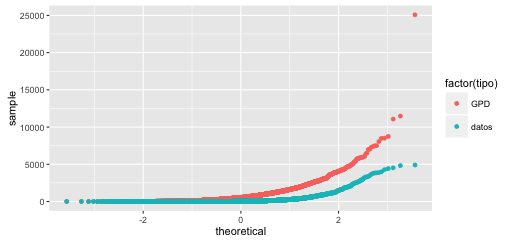
\includegraphics[width=35mm]{6gevf.png}} &
       \addheight{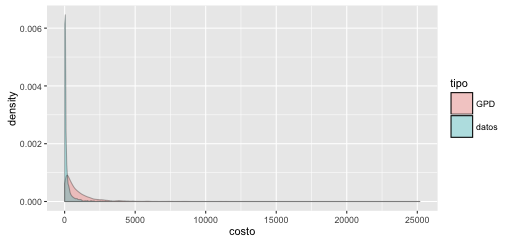
\includegraphics[width=35mm]{6gevf_dens.png}} \\
       \hline
      \addheight{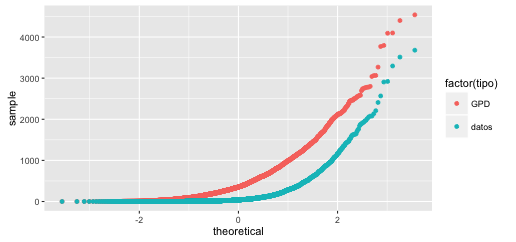
\includegraphics[width=35mm]{7gev.png}} &
      \addheight{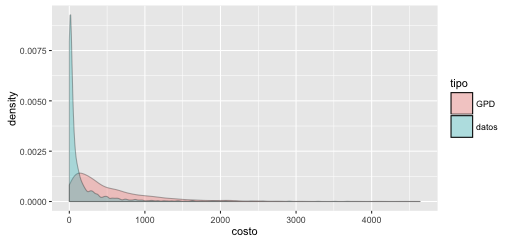
\includegraphics[width=35mm]{7gevf_dens.png}} \\
      \hline
\end{tabular}\\
\noindent En la tabla anterior se ven las distribuciones de valores extremos generalizados ajustadas con el m\'etodo de m\'axima verosimilitud dados nuestros datos separados por a\~{n}o comparadas con la distribuci\'on emp\'irica de los mismos (qq-plot e histogramas suavizados). Aunque parece que las distribuciones ajustadas siguen el mismo comportamiento de los datos, existen ciertas regiones de las mismas que se alejan bastante de los valores emp\'iricos de la distribuci\'on. Dado que tenemos m\'as de 2500 datos para ajustar cada modelo, estas separaciones entre distribuci\'on ajustada y distribuci\'on empirica nos podr\'ian hacer pensar que podemos mejorar tomando otro enfoque.
\begin{itemize}
\item Se ajustaron modelos para 2005, 2006 y 2007 tanto de una distribuci\'on de valores extremos generalizados, como de una funci\'on de distribuci\'on pareto generalizada.
\item Las gr\'aficas de estos ajustes y los m\'etodos de selecci\'on de el mejor modelo se ver\'an en la secci\'on 2.3 .
\item La gr\'afica de abajo muestra un caso en particular (2007) donde la distribuci\'on ajustada pareto generalizada (rojo) no parece tener la misma distribuci\'ion que nuestros datos (azul).
\end{itemize}
%\begin{description}
%\item[First] This is the first item
%\item[Last] This is the last item
%\end{description}
\begin{tabular}{|c|}
      \hline
      \addheight{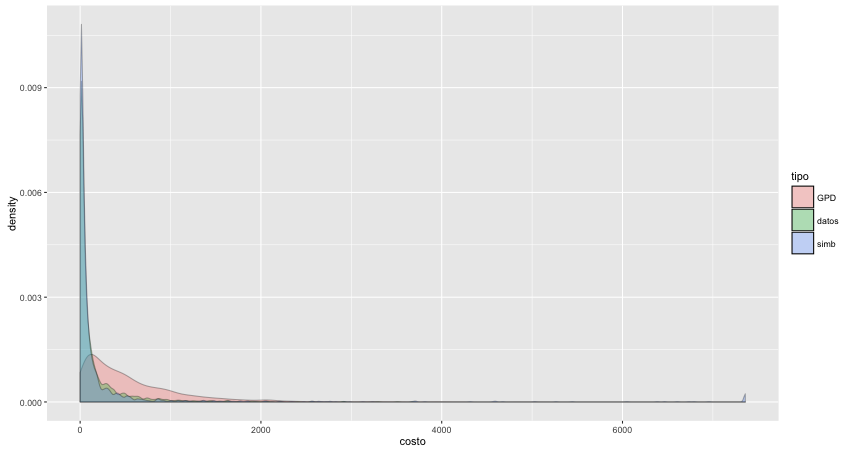
\includegraphics[width=75mm]{comparacion_dens_p7.png}} \\
      \hline
\end{tabular}

\subsection{Enfoque bayesiano}
\indent {\small{Para el segundo enfoque utilizaremos el paquete evdbayes de R adem\'as de otros paquetes como ggplot2 para graficar los resultados. }}
%\lipsum[9] % Dummy text
\begin{tabular}{|c|}
      \hline
      \addheight{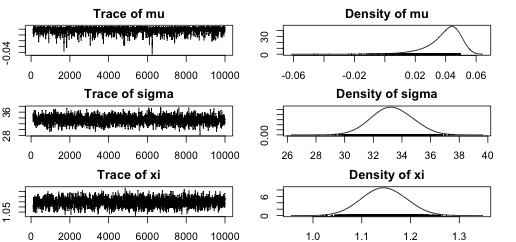
\includegraphics[width=60mm]{theta_5.png}} \\
      \hline
       \addheight{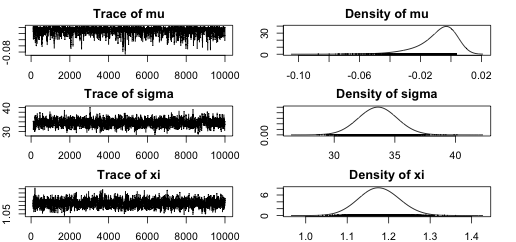
\includegraphics[width=60mm]{theta_6.png}} \\
       \hline
      \addheight{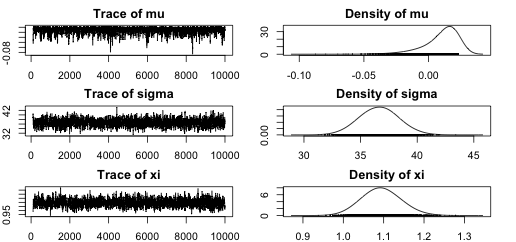
\includegraphics[width=60mm]{theta_7.png}} \\
      \hline
\end{tabular}

\begin{itemize}
\item Tomamos distribuciones no informativas como a priori (normales (0,10000)).
\item En el enfoque bayesiano simulamos diferentes distribuciones para los par\'ametros de cada distribuci\'on.
\item En la tabla de arriba se ven las simulaciones y las distribuciones emp\'iricas de los 3 par\'ametros  de una distribuci\'on de valores extremos o pareto generalizadas.
\item De nuevo, se calcularon modelos para cada a\~{n}o  de una distribuci\'on pareto generalizada y de una distribuci\'on de valores extremos generalizados.
\end{itemize}


\begin{tabular}{|c|}
      \hline
      \addheight{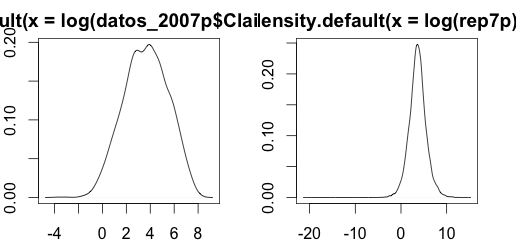
\includegraphics[width=75mm]{dens_log_bpar_7.png}} \\
      \hline
\end{tabular}
\noindent Comparaci\'on de las densidades del logaritmo de los datos del 2007 contra el logaritmo de nuestro ajuste simulado para 2007.
\subsection{Selecci\'on del Modelo}
%-------------------------------------------------
\begin{tabular}{|c|}
      \hline
      \addheight{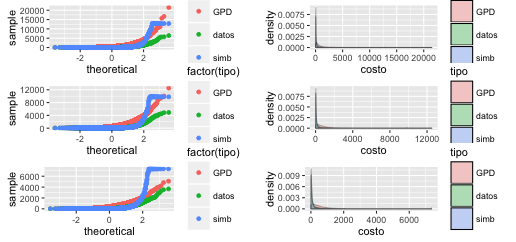
\includegraphics[width=75mm]{comparacion_qq_dens_anual.png}} \\
      \hline
\end{tabular}

\begin{itemize}
\item Los modelos que se hicieron con distribuciones pareto generalizadas siempre ajustaron mejor que los modelos que se hicieron con distribuciones de valores extremos generalizados.
\item Esto ocurri\'o tanto para el enfoque frecuentista como el bayesiano.
\item La comparaci\'on se hizo con AIC y log-verosimilitud.
\item Para comparar al modelo bayesiano contra el frecuentista decidimos usar el qq-plot y m\'etodos gr\'aficos ya que observamos que los valores que hac\'ian que el modelo bayesiano perdiera eran los valores extremos de la distribuci\'on (los cuales terminamos acotando gracias a teor\'ia que encontramos de sucesos catastr\'oficos).
\end{itemize}

\begin{tabular}{|c|}
      \hline
      \addheight{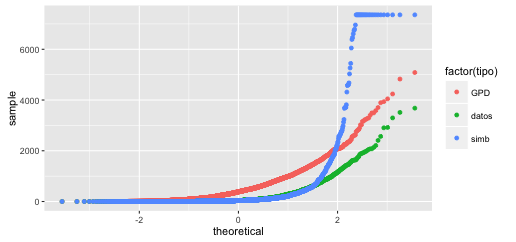
\includegraphics[width=70mm]{comparacion_qq_7fb.png}} \\
      \hline
       \addheight{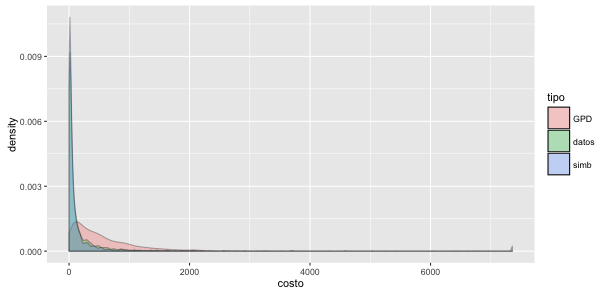
\includegraphics[width=70mm]{comparacion_dens_7fb.png}}\\
      \hline
      \hline
\end{tabular}\\
\begin{itemize}
\item En general, los valores que optimizaron los criterios de AIC y log-verosimilitud (BIC para los bayesianos) fueron los del modelo pareto generalizado frecuentista, sin embargo por las gr\'aficas y gracias a la cota que pusimos sobre el modelo bayesiano creemos que es mejor para el ajuste. 
\end{itemize}

\section{Simulaci\'on y Teor\'ia de Ruina}

\begin{tabular}{|c|c|}
      \hline
      \addheight{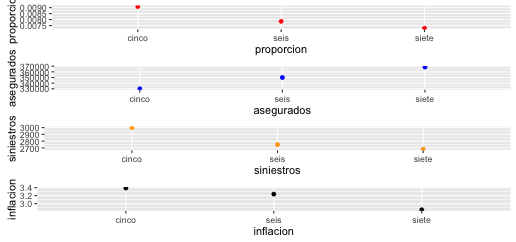
\includegraphics[width=35mm]{datos_anuales_N.png}} &
       \addheight{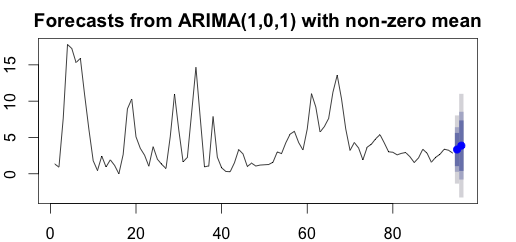
\includegraphics[width=35mm]{inflation.png}}\\
      \hline
      \hline
\end{tabular}\\

\begin{tabular}{|c|}
	\hline
  	\addheight{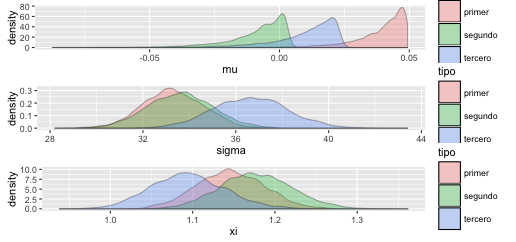
\includegraphics[width=75mm]{theta_comparacion_anual.png}}\\
	\hline
\end{tabular}

\begin{itemize}
\item Para simular de nuestro modelo bayesiano (todo un problema) decidimos hacer una mezcla de los 3 modelos para cada par\'ametro d\'andole mayor importancia al del 2007, despu\'es al del 2006 y tomando como de menor importancia a la distribuci\'on de los par\'ametros del a\~{n}o 2005.
\item Por la forma de las distribuciones de los par\'ametros (tabla de arriba), creemos que tomar el enfoque bayesiano no es mala idea (dado que estas distribuciones a veces no son ni siquiera sim\'etricas). Esto lo explicamos como que existe mucha informaci\'on de los datos que no estar\'iamos explicando sin este modelo. 
\item Simulamos con la mezcla de los siniestros y con una N \~ Poisson con intensidad creada de manera lineal de las intensidades anteriores. Para cada N generamos $n_i$ X distribuidas con la mezcla de los modelos para los par\'ametros y pareto generalizadas para x.
\item Para ver cu\'al era la probabilidad de ruina de cierto $\theta$, $U_0$ y datos, simulamos una muestra de 1000 N para cada a\~{n}o y para cada n simulamos sus respectivos tiempos entre siniestros para crear un proceso de saltos que "compitiera" con el capital inicial y la prima planeada creciendo de manera lineal en el a\~{n}o (ver c\'odigo en R para entender mejor).
\end{itemize}
%---------------------------------------------------
%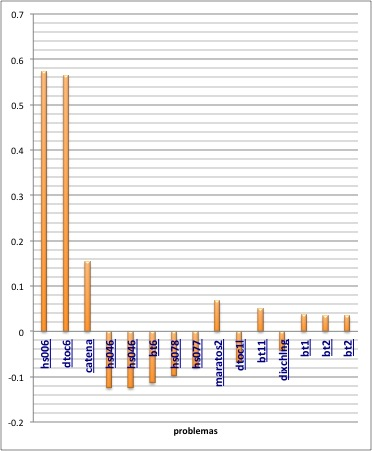
\includegraphics[trim = 0mm 0mm 00mm 0mm, clip, scale=1.2]{rendimiento(feval).jpg}\\
\section{Conclusiones}

\begin{tabular}{|c|}
	\hline
  	\addheight{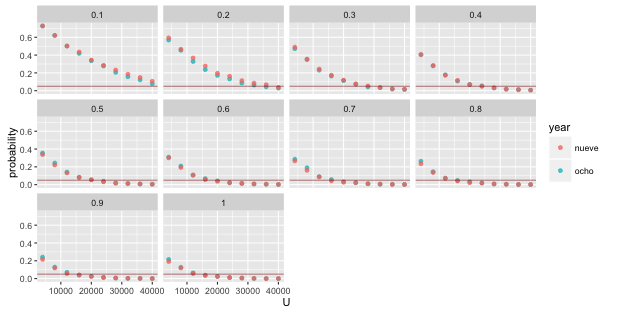
\includegraphics[width=75mm]{ruina.png}}\\
	\hline
\end{tabular}

\begin{description}
\item[Probabilidades] En la tabla de arriba se muestran para diferentes valores de $\theta$ y de $U_0$ las probabilidades simuladas de ruina en los dos a\~{n}os.
\item[Primas] Para cada valor de $\theta$ y cada valor de capital inicial $U_0$ se tiene una prima que genera una probabilidad de ruina menor a 0.05 (marcada por la l\'inea roja).
\item[Predicci\'on] Nuestro enfoque fue evitar la ruina tomando una prima (o un capital inicial) que nos dejara con una probabilidad de 0.05 de fracaso.  
\end{description}
%----------------------------------------------------------------------------------------
%	REFERENCE LIST
%----------------------------------------------------------------------------------------

%\begin{thebibliography}{99} % Bibliography - this is intentionally simple in this template
%
%\bibitem[Figueredo and Wolf, 2009]{Figueredo:2009dg}
%Figueredo, A.~J. and Wolf, P. S.~A. (2009).
%\newblock Assortative pairing and life history strategy - a cross-cultural
%  study.
%\newblock {\em Human Nature}, 20:317--330.
% 
%\end{thebibliography}
%\bibitem[Coles S, 2001]{Modeling}
%Coles S. (2001).
%\newblock An Introduction to Statistical Modeling of Extreme Values.
%\newblock {\em Springer, 1st edition}
%
%% \bibitem[Denuit M, 2008]{Risk}
%%Denuit Michel, Dhaene Jan, Goovaerts Marc, Kaas Rob .(2008).
%%\newblock Modern Actuarial Risk Theory.
%%\newblock {\em Springer, 2nd edition}
%%
%% \bibitem[Gilleland E,  2009]{Conference}
%%Eric Gilleland .(22 June 2009).
%%\newblock An introduction to the analysis of extreme values using R and extRemes .
%%\newblock {\em 6th International Conference on Extreme Value Analysis}
%
%\end{thebibliography}
%https://cran.r-project.org/web/packages/evdbayes/evdbayes.pdf
%
%https://finzi.psych.upenn.edu/library/evdbayes/doc/guide.pdf
%
%Coles S. An Introduction to Statistical Modeling of Extreme Values. Springer, 1st edition, 2001.
%
%Denuit Michel, Dhaene Jan, Goovaerts Marc, Kaas Rob. Modern Actuarial Risk Theory. Springer, 2 edition, 2008.								
%
%Eric Gilleland, An introduction to the analysis of extreme values using R and extRemes . Graybill VIII, 6th International Conference on Extreme Value Analysis 22 June 2009 .

%----------------------------------------------------------------------------------------

\end{document}